\documentclass[12pt]{article}

\usepackage{sbc-template}

\usepackage{graphicx,url}

\usepackage[brazil]{babel}   
%\usepackage[latin1]{inputenc}  
\usepackage[utf8]{inputenc}  
% UTF-8 encoding is recommended by ShareLaTex
\usepackage{multicol}
\usepackage[none]{hyphenat}
\newenvironment{Figure}
  {\par\medskip\noindent\minipage{\linewidth}}
  {\endminipage\par\medskip}     
\sloppy

\usepackage{listings}
\usepackage{xcolor}
\lstset { %
    language=C,
    %backgroundcolor=\color{black!5}, % set backgroundcolor
    basicstyle=\tiny,% basic font setting
}

\title{Relatório de Entrega de Trabalho \\
       %Disciplina de programação Paralela (PP) \\ Prof. César De Rose \\
       Exercício 1}

\author{Leonardo G. Carvalho(pp12816), Matheus S. Redecker(pp12819)}


%\address{Pontifícia Universidade Católica do Rio Grande do Sul - PUCRS
%  \email{  \{leonardo.gubert\}\{matheus.redecker\} @acad.pucrs.br}
%}


\begin{document} 

\maketitle

{\footnotesize
\begin{multicols}{2}
\section{Introdução}
O objetivo deste trabalho é, utilizando a biblioteca MPI, implementar uma versão paralela de um programa que realiza a ordenação de linhas de uma matriz através do algoritmo de \textit{Quick Sort} utilizando o modelo mestre e escravo. A modelagem do problema foi feita pensando que os escravos precisam receber uma linha da matriz, realizar a ordenação e enviar de volta para o mestre a linha ordenada. Para isso ser realizado foi definido o ultimo processo como sendo o mestre, e os demais processos como escravos. 

\section{Implementação}
Quando o mestre é executado, a primeira coisa a ser feita é criar e alocar memória para a matriz principal. Feito isso, o mestre realiza um \textit{burst} inicial, enviando para cada um dos escravos uma linha da matriz com uma \textit{tag} identificando qual a posição da linha que foi enviada. Após todos os escravos receberem uma linha, o mestre entra em um laço onde ele espera que qualquer escravo mande de volta a linha ordenada. Quando a mensagem é recebida, é feito um \textit{MPI\_Probe} para atualizar as informações de \textit{tag} e assim é feito um \textit{MPI\_Recv} endereçando o bloco recebido diretamente na linha correspondente através da informação da \textit{tag}. Se ainda existirem linhas a serem ordenadas, a próxima da sequencia é enviada para este escravo, senão, o mestre manda uma mensagem para finalizar o processo do escravo. Este laço do mestre é executado até que todas as linhas enviadas tenham sido recebidas ordenadas.\\Para o escravo a tarefa é mais simples: A primeira coisa a ser feita é alocar memoria para o vetor que deve ser ordenado. Após isso o escravo entra em um laço onde ele recebe uma linha da matriz e verifica se a \textit{tag} não é para finalizar o processo. Se for, ele é finalizado, senão ele faz a ordenação da linha e a envia para o mestre.

\section{Dificuldades encontradas}
Inicialmente não estávamos utilizando a função \textit{MPI\_Probe}, fazendo com que a \textit{tag} lida não fosse a correta no momento da resposta do escravo para o mestre com o vetor ordenado.

\section{Testes}
Os testes foram executados com a alocação de 2 nodos no cluster Atlantica. A execução paralela foi executada utilizando 2, 3, 5, 7, 9, 17 processos paralelos. Tirando a execução com 2 processos, a quantidade de processos foi impar pelo fato de que um dos processos é o mestre, então o restante é quem realmente realiza a ordenação da matriz, o único caso par foi utilizado para representar o programa sequencial, um sendo mestre e um escravo. A matriz foi definida como sendo 1.000x100.000 (mil linhas por cem mil colunas) números gerados através de uma função que cria o pior caso para a ordenação par o algoritmo de \textit{Quick Sort}.

\section{Análise de desempenho}
A versão paralela obtém um desempenho superior ao da sequencial quando o número de processos é pequeno. A medida que o número vai aumentando o desempenho estabiliza e após isso diminui. A figura abaixo apresenta o gráfico que demonstra este comportamento. A partir do comportamento do desempenho foi possível analisar que o algoritmo do \textit{Quick Sort} é tão rápido que realiza a ordenação do vetor rapidamente, as trocas de mensagens entre os escravos e os mestres acabam consumindo mais tempo do que a ordenação, com isso quando são adicionados mais escravos não há mais muito ganho de desempenho como no inicio, fazendo até com que o programa perca desempenho quando adicionados mais escravos, isso acontece por conta do \textit{overhead} da troca de mensagens, ou seja, do tempo que o mestre precisa para enviar mais mensagens para mais escravos não compensa o trabalho realizado.
\begin{Figure}
\centering
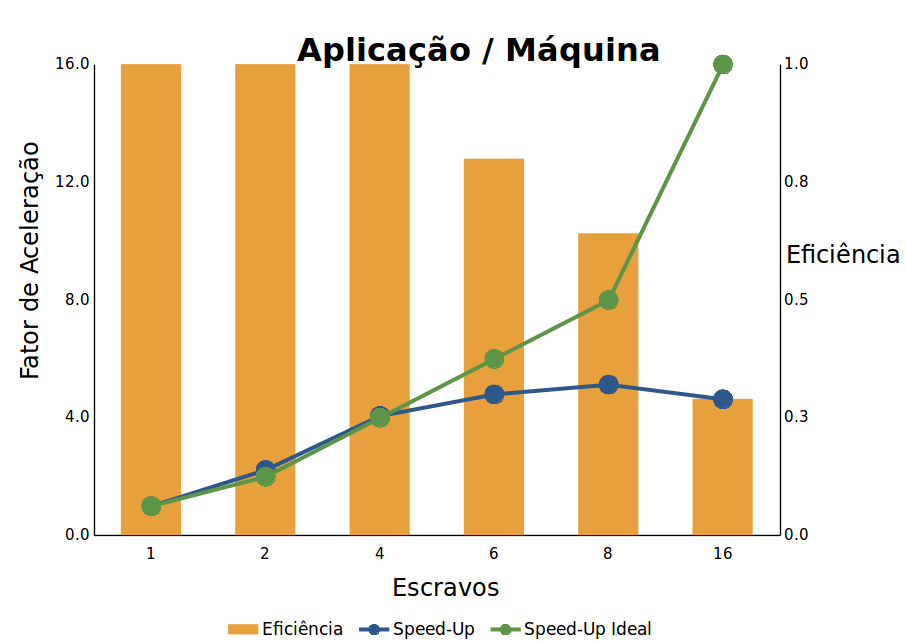
\includegraphics[width=\columnwidth]{fig/graficot1.png}
\label{fig:grafico}
\end{Figure}
\section{Observações finais}
O que podemos concluir é que este problema possui um melhor desempenho quando utilizado em paralelo, mas devido ao alto desempenho do algoritmo de ordenação e ao mecanismo de pilha do MPI, não há um ganho muito grande quando são adicionados mais escravos, pelo fato do \textit{overhead} da troca de mensagens que acaba afetando o desempenho de forma negativa.
\end{multicols}

\newpage{}
\section{Código}

}
%{\scriptsize \tiny %LEO TESTA COM ESSE AQUI E VÊ QUE TU ACHA PORQUE DAI CABE EM UMA PAGINA
%\begin{verbatim}
\begin{lstlisting}
#include <stdio.h>
#include <stdlib.h>
#include "mpi.h"

#define MATRIX_LINES 1000
#define MATRIX_COLUMNS 100000
#define SUICIDE_TAG 666666

int *theMatrix[MATRIX_LINES];
int *slaveBuffer;

void createMatrix()
{
   //Aloca a matriz
    int i, j;
    for (i = 0; i < MATRIX_LINES; i++){
        theMatrix[i] = malloc(sizeof(int) * MATRIX_COLUMNS);
    }
   //Preenche
    for (i = 0; i < MATRIX_LINES; i++){
        for(j = 0; j<MATRIX_COLUMNS; j++){
            theMatrix[i][j] = MATRIX_COLUMNS - j + (10*i);
        }
    }
}

int main(int argc, char** argv)
{
    int my_rank;  // Identificador do processo
    int proc_n;   // Numero de processos
    int nextVector; //Qual a posicao do proximo vetor a ser enviado
    int receivedVectors; // Quantos vetores ja foram recebidos 
    MPI_Status status; // Status de retorno

    MPI_Init (&argc, &argv);

    MPI_Comm_rank(MPI_COMM_WORLD, &my_rank);
    MPI_Comm_size(MPI_COMM_WORLD, &proc_n);
    
    //MESTRE
    if (my_rank == proc_n-1){
	    //utilizado para contagem do tempo
	    double t1,t2;
	    t1 = MPI_Wtime();
        //Cria a matriz original
        createMatrix();

        //Faz a distribuicao inicial
        for(nextVector = 0; nextVector < proc_n-1; nextVector++){
            MPI_Send(theMatrix[nextVector], MATRIX_COLUMNS,
            MPI_INT, nextVector, nextVector, MPI_COMM_WORLD);
        }

        // Enquanto ainda ha linhas a serem ordenadas
        while(receivedVectors<MATRIX_LINES){
            //Recebe a linha ordenada
            //e envia outra para o mesmo escravo
            MPI_Probe(MPI_ANY_SOURCE, MPI_ANY_TAG, 
                      MPI_COMM_WORLD, &status);
            MPI_Recv (theMatrix[status.MPI_TAG], MATRIX_COLUMNS,
                      MPI_INT, MPI_ANY_SOURCE, MPI_ANY_TAG,
                      MPI_COMM_WORLD, &status);
            receivedVectors++;

            //Se ainda ha vetores a serem enviados, manda ele.
            if(nextVector<MATRIX_LINES) {
                MPI_Send (theMatrix[nextVector], MATRIX_COLUMNS,
                          MPI_INT, status.MPI_SOURCE,
                          nextVector, MPI_COMM_WORLD);
                nextVector++;
            }
            //se nao manda o processo finalizar
            else{
                int nada = 10;
                MPI_Send (&nada, 1, MPI_INT, status.MPI_SOURCE,
                          SUICIDE_TAG, MPI_COMM_WORLD);
            }
        }
	    t2 = MPI_Wtime(); // termina a contagem do tempo
    }
    //ESCRAVOS
    else {
        //Inicializa o buffer
        slaveBuffer = malloc(sizeof(int) * MATRIX_COLUMNS);
        while(1){
            MPI_Recv (slaveBuffer, MATRIX_COLUMNS, MPI_INT, 
                      proc_n-1, MPI_ANY_TAG, MPI_COMM_WORLD,
                      &status);
            if(status.MPI_TAG == SUICIDE_TAG){
                break;
            }
            //Faz a ordenacao no vetor e retorna para o mestre
            qsort(slaveBuffer, MATRIX_COLUMNS, sizeof(int), cmpfunc);
            MPI_Send (slaveBuffer, MATRIX_COLUMNS, MPI_INT,
                      proc_n-1, status.MPI_TAG, MPI_COMM_WORLD);
        }
    }
    MPI_Finalize();
}
\end{lstlisting}
%\end{verbatim}}
\end{document}
